\begin{problem}{Extreme Sort}{standard input}{standard output}{sort}

John likes sorting algorithms very much. He has studied quicksort, merge sort, radix sort, and many
more.\\
A long time ago he has written a lock-free parallel string sorting program. It was a combination
of burstsort and multi-key quicksort. To implement burstsort you need to build a tree of buckets.\\
For each input string you walk through the tree and insert part of the string into the right bucket.
When a bucket fills up, it ``bursts'' and becomes a new subtree (with new buckets).

\begin{center}
  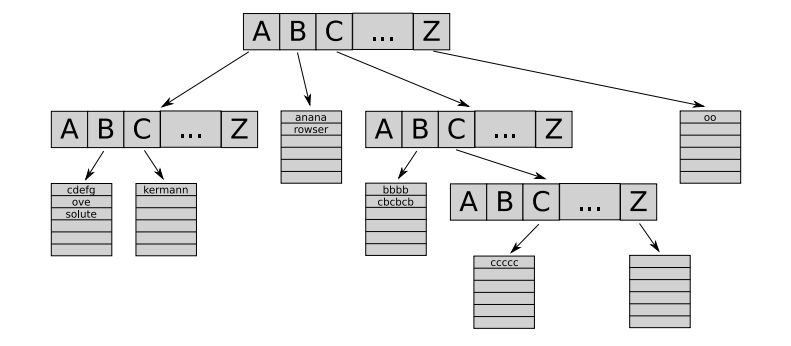
\includegraphics[scale=0.6]{./texts/src/d1.png}\\
  Figure D-1: Burstsort data structure.
\end{center}

Well, enough about the past. Today John is playing with sorting algorithms again. This time it’s
numbers. He has an idea for a new algorithm, ``extreme sort''. It’s extremely fast, performance
levels are OVER NINETHOUSAND. Before he tells anyone any details, he wants to make sure
that it works correctly.\\
Your task is to help him and verify that the so-called extreme property holds after the first phase
of the algorithm. The extreme property is defined as $min (x_{i,j}) \geq 0$, where

\begin{center}
  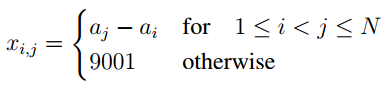
\includegraphics[scale=0.5]{./texts/src/d2.png}\\
\end{center}

\InputFile

The first line contains a single integer $N\ (1 \leq N \leq 1024)$. The second line contains $N$
integers $a_1\ a_2\ .\ .\ .\ a_N\ (1 \leq a_i \leq 1024)$.

\OutputFile

Print one line of output containing ``yes'' if the extreme property holds for the given input,
``no'' otherwise.

\Example

\begin{example}
\exmp{
2
1 2
}{
yes
}%
\exmp{
4
2 1 3 4
}{
no
}%
\end{example}

\end{problem}
